 \documentclass{article}

% if you need to pass options to natbib, use, e.g.:
% \PassOptionsToPackage{numbers, compress}{natbib}
% before loading nips_2016
%
% to avoid loading the natbib package, add option nonatbib:
% \usepackage[nonatbib]{nips_2016}

\usepackage[final,nonatbib]{../LaTeXStyleFiles/nips_2016}

% to compile a camera-ready version, add the [final] option, e.g.:
% \usepackage[final]{nips_2016}

\usepackage[utf8]{inputenc} % allow utf-8 input
\usepackage[T1]{fontenc}    % use 8-bit T1 fonts
\usepackage[colorlinks]{hyperref}       % hyperlinks
\usepackage{url}            % simple URL typesetting
\usepackage{booktabs}       % professional-quality tables
\usepackage{amsfonts}       % blackboard math symbols
\usepackage{nicefrac}       % compact symbols for 1/2, etc.
\usepackage{microtype}      % microtypography
\usepackage{amsmath}
\usepackage{tikz}
\usetikzlibrary{positioning}
\usetikzlibrary{shapes.geometric}
\usetikzlibrary{calc}
\usetikzlibrary{circuits.logic.US}

\tikzset{
  multiplexer/.style={
    draw,
    trapezium,
    shape border uses incircle, 
    shape border rotate=270,
    minimum size=18pt
  }
}

\newcommand{\code}[1]{\texttt{#1}}

\bibliographystyle{ieeetr}

\title{Project Proposal}

% The \author macro works with any number of authors. There are two
% commands used to separate the names and addresses of multiple
% authors: \And and \AND.
%
% Using \And between authors leaves it to LaTeX to determine where to
% break the lines. Using \AND forces a line break at that point. So,
% if LaTeX puts 3 of 4 authors names on the first line, and the last
% on the second line, try using \AND instead of \And before the third
% author name.

\author{
    Kyle~Daruwalla \\
    Department of Electrical and Computer Engineering \\
    University of Wisconsin -- Madison \\
    \texttt{daruwalla@wisc.edu} \\
    \And
    Akhil~Sundararajun \\
    Department of Electrical and Computer Engineering \\
    University of Wisconsin -- Madison \\
    \texttt{asundararaja@wisc.edu} \\
}

\begin{document}

\maketitle

% Each section (including abstract) has its own .tex file
% The name of the .tex file corresponds to the section title
% e.x. The subsection in the Introduction on FPGAs is called
%      intro-fpga.tex
% \input{filename} is equivalent to pasting in the raw text
% from filename.tex.
% Try to edit the filename.tex files and not proposal.tex.
% This avoids conflicts most of the time.

\section{Introduction}
\textit{Include brief information on setting up the CNN problem.}
Testing

\subsection{Field-Programmable Gate Arrays}
\textit{Include brief information on FPGAs.}

\section{Design Methodology}
In order to perform an effective comparison between software implementations of CNNs and hardware implementations, we propose using TensorFlow, Amazon EC2, and Xilinx FPGAs. TensorFlow will be used to implement various software implementations of a given CNN structure for ImageNet. These CNN implementations will be trained and tested on Amazon EC2. A hardware implementation of the CNN will be created for Xilinx FPGAs in Vivado. Simulations will be performed to verify its functionality, and it will be deployed on a physical FPGA to test its timing characteristics and accuracy.
\subsection{TensorFlow Baseline}
The first experiment will be to study training performance of the ImageNet dataset on Amazon EC2, which will serve as a baseline for a traditional single-machine CPU setting.  We propose to use TensorFlow, an open-source, python-based machine learning package released by Google in November 2015 \cite{tensorflow}.  In addition, using packages in TensorFlow, we will study GPU acceleration on Amazon EC2.  Due to TensorFlow’s distributed execution capability, we also propose to train CNNs using the {\sc{Hogwild!}} algorithm.  Since SGD is inherently serial, our FPGA implementation targets lowering cost per iteration.  This can be compared to {\sc{Hogwild!}}, which is a parallelized approach to achieving speedup.  Due to the variety of structural and parameter design choices typical in building a CNN, we also propose to examine several CNN architectures in combination with the different hardware platforms considered in this project.  Different activation functions including sign, ReLU, and sigmoid also will be explored.

\subsection{Convolutional Neural Networks on FPGAs}
Each filter in the CNN will be modeled as a \textit{unit-neuron} on the FPGA (shown in Figure \ref{fig:unit-neuron}). During the compute phase, the selector signal $s$, will feed the current patch $(x_0, x_1, x_2, x_3, x_4)$ into the unit-neuron. A weight register file will hold the current weights, $(w_0, w_1, w_2, w_3, w_4)$. The activation function, $\sigma$, will be approximated using a lookup table if it is not piecewise linear. The output $f$ will store a single pixel of output for a given filter.
\begin{figure}[hb]
	\centering
	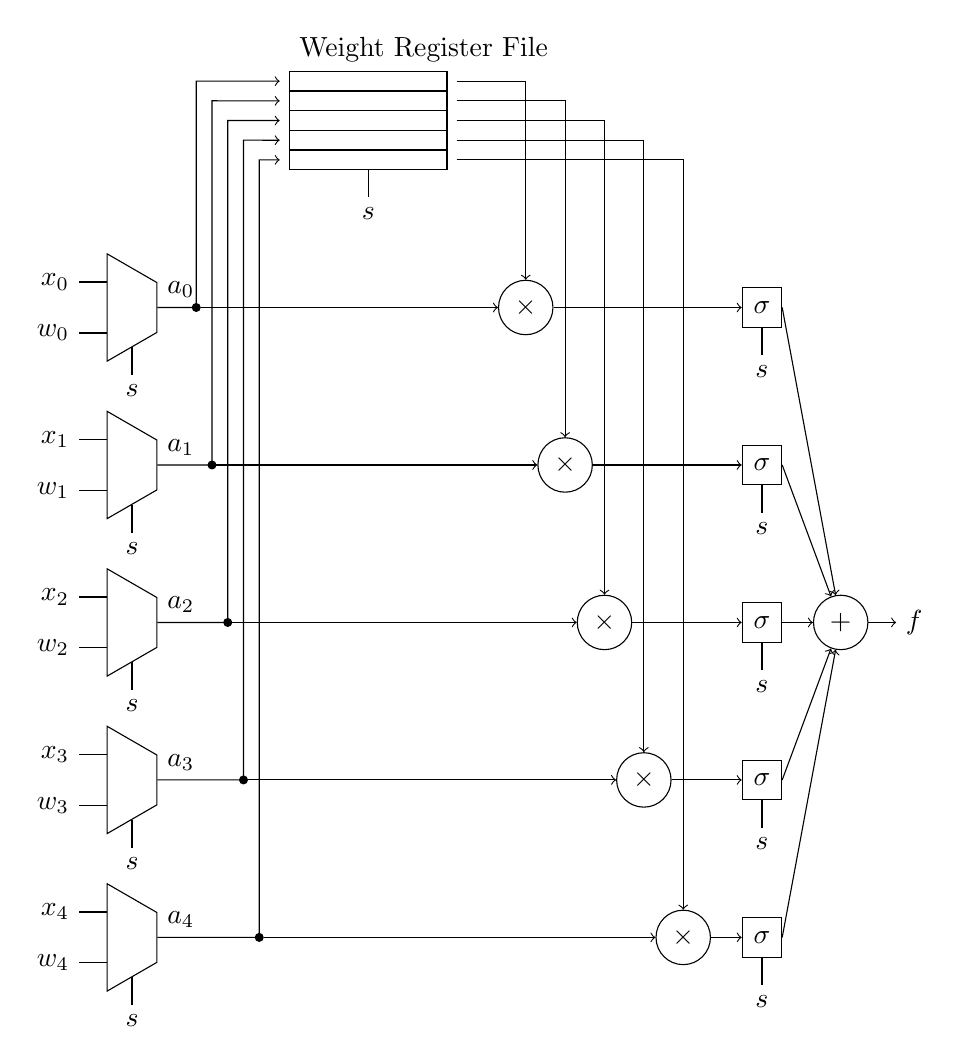
\begin{tikzpicture}
		\foreach \i in {0, ..., 4} {
			\node[multiplexer] (mux\i) at (0, -2*\i) {};
			\draw (mux\i.north west) --++ (-10pt, 0) node [left] {$x_\i$};
			\draw (mux\i.south west) --++ (-10pt, 0) node [left] {$w_\i$};
			\draw (mux\i.south) --++ (0, -10pt) node [below] {$s$};
		}

		\draw (2, 3) node[above right] {Weight Register File} rectangle (4, 1.75);
		\draw (3, 1.75) --++ (0, -10pt) node[below] {$s$};
		\foreach \i in {0, ..., 4} {
			\draw ($(2, {2.75-0.25*\i})$) node[above] (wrf\i) {} --++ (2, 0) node[above] (wrf\i-out) {};
			\draw [->] (mux\i.top side) node [above right] {$a_\i$} --++ (14pt, 0) --++ (0.2*\i, 0) node[circle, fill, draw, inner sep=-1pt] (junc\i) {} --++ ($(0, 2.875+1.75*\i)$) -- (wrf\i);
		}

		\foreach \i in {0, ..., 4} {
			\node[circle, draw] (mul\i) at ($(5+0.5*\i, -2*\i)$) {$\times$};
			\draw [->] (junc\i) -- (mul\i.west);
			\draw [->] (wrf\i-out) --++ ($(1+0.5*\i, 0)$) -- (mul\i.north);
		}

		\node[circle, draw] (sum) at (9, -4) {$+$};

		\foreach \i in {0, ..., 4} {
			\node[rectangle, minimum height=0.5cm, minimum width=0.5cm, draw] (sigma\i) at ($(8, -2*\i)$) {$\sigma$};
			\draw [->] (mul\i.east) -- (sigma\i.west);
			\draw [->] (sigma\i.east) -- (sum);
			\draw (sigma\i.south) --++ (0, -10pt) node[below] {$s$};
		}

		\draw [->] (sum.east) --++ (10pt, 0) node[right] {$f$};
	\end{tikzpicture}
	\caption{A unit-neuron implementation for an FPGA with a filter size of 5}
	\label{fig:unit-neuron}
\end{figure}

A controller will adjust $(x_0, x_1, x_2, x_3, x_4)$ so that it corresponds to the current patch being evaluated. After the compute phase is complete, it will update the $(w_0, w_1, w_2, w_3, w_4)$ values and drive $s$ high so that the weight register file can be updated. There will be latching (not shown in Figure \ref{fig:unit-neuron}) on the output values of the filters so that they can be held while the weights are updated.

The potential for speedup comes from parallelizing the filter operation, using faster fixed-point computation units, and approximation of the activation function.
\subsection{MATLAB Verification}
While our hardware implementation is serially equivalent to a traditional software implementation for a CNN, it does use limited precision. We implemented a limited precision CNN model of the hardware in MATLAB to verify its convergence.

This was achieved by using a custom quantization function to limit the precision of the numbers used by MATLAB. Using a custom function allowed us to have tight control of the rounding scheme, and it is faster than using the object-oriented fixed-point model in MATLAB.

Similar to the TensorFlow and hardware, the MATLAB simulation is also trained using mini-batch stochastic gradient descent with a batch size of 128 (same as TensorFlow). The purpose of this simulation was to emulate training the hardware on the same dataset as TensorFlow verify the hardware's convergence. It was not intended to be used for a timing comparison.

\section{Results}
After creating an FPGA implementation of a neural network, timing characteristics for a particular CNN can be created. For example, the proposed unit-neuron will have some physical path delay, $\tau$. Using this known constant and the structure of our CNN, we would like to define a design space. This will allow a designer targeting neural networks on FPGAs to know the time per iteration as a function of $\tau$, the number of layers, and the CNN structure. This will provide some theoretical closed form for the computational complexity on an FPGA.

Additionally, after collecting empirical results, we would like to do perform the following analysis:
\begin{enumerate}
	\item Comparing generalization error between the CPU, GPU, {\sc{Hogwild!}}, and FPGA implementations.
	\item Comparing convergance rates (in terms of seconds) for SGD with backprop between the CPU, GPU, {\sc{Hogwild!}}, and FPGA implementations.
	\item Provide a metric of when FPGAs might provide a larger speedup than {\sc{Hogwild!}}
\end{enumerate}


\section{Conclusion}
Our results show that FPGAs are a viable option for speeding up the training phase for CNNs. However, we also note that these implementations are constrained by the resources available, and thus, FPGA implementations are only useful if the network can be partitioned. In particular, training a small to medium sized networks on a single CPU or GPU is likely a better option than an FPGA implementation. However, as the input data and the network depth scales up, the benefits of CPU implementations fail to deliver speed-up. Particularly, at the scale of data centers like Microsoft \cite{project-catapult}, an FPGA implementation offers the necessary speed-up while still being more power efficient than an equivalent GPU offering.

Furthermore, our loss convergence results illustrate the need to explore limited precision training more deeply. Currently, neural network designers add controlled noise to the data or model (via dropout) in order to increase the model robustness. We would like to explore using quantization error to introduce this noise. The properties of quantization error can be controlled and bounded via varying rounding schemes. Moreover, the benefits of quantization and limited precision are two-fold -- first, controlled noise can make the model more robust if inserted intelligently; second, the reduced bit length leads to faster hardware and more resources on-chip to create parallel execution units.

In summary, this project illustrates a promising direction for further exploration. In the future, we would like to implement partitioning networks across several FPGAs to increase the clock frequency and number of parallel execution units, as well as understand the effects of quantization and limited precision on the robustness of CNNs. We conclude that FPGAs are a suitable candidate for speed-up when the networks and datasets are sufficiently large, and when aggregate power consumption is costly.

\newpage
\nocite{*}
\bibliography{references}

\end{document}
